\chapter{The Standard Model and Beyond}
\label{chap:theory}

The Standard Model of particle physics describes all
known fundemental particles and the interactions between them (with the exception
of the gravitational force). Developed over decades in the latter half of the 20$^\mrm{th}$
century, it has predicted experimental findings to an extraordinary degree of accuracy,
and represents one of the crowning achievements of modern science.
However, despite it successes, there are a number of known phenomena that cannot be
explained with the current theory, giving physicists reason to look for an expanded model.
In this chapter, we outline the Standard Model as it currently exists, discuss some
of the challenges that the model faces, and give a brief survey of proposed extensions to
the Standard Model that are relevant to this thesis.


\section{The Standard Model of particle physics}

The Standard Model (SM) is at its core a quantum field theory defined by a local 
$SU(3)\times SU(2)\times U(1)$ gauge symmetry. We will explain what exactly this means shortly 
(basically, each term gives rise to one of the three fundamental interactions), but for now we simply
describe all of the known particles and their properties.

\begin{figure}[ht]
  \begin{center}
    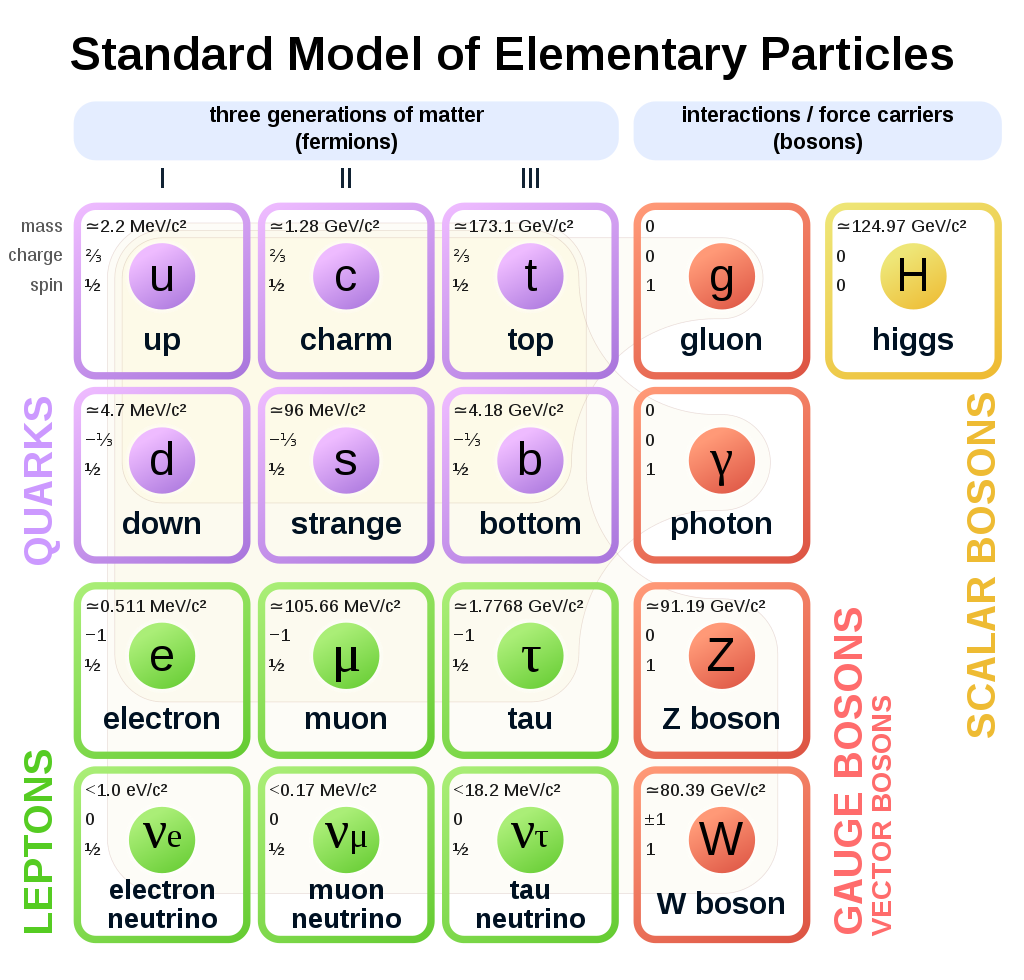
\includegraphics[width=0.70\textwidth]{figs/theory/standard_model.png}
    \caption{Diagram of all fundemental particles making up the Standard Model. There are 12 fermions (spin-\nicefrac{1}{2}), 
      consisting of six quarks (purple) and six leptons (green), 
      and divided into three generations. There are additionally four force-carrying vector bosons (spin-1),
      that couple to the fermions and give rise to the strong, weak, and electromagnetic interactions.
      Finally, the scalar Higgs boson, proposed in 1964 and discovered in 2012, provides the mechanism
      by which the other particles acquire mass. (Taken from \cite{SM_diagram})
            }
    \label{fig:sm}
  \end{center}
\end{figure}

\subsection{Fundamental particles}

Figure~\ref{fig:sm} shows all distinct particles in the SM, organized into groups.
On the left, in purple and green, are the 12 fundamental fermions, defined by the
value of their intrinsic angular momentum, or ``spin'', of \nicefrac{1}{2} (in units
of $\hbar$). By the spin-statistics theorem, fermions obey the Pauli exclusion principle,
meaning no two can occupy the same quantum state simultaneously.

The fermions are further defined by the various charges they carry (which determine how they
interact with the bosons, as we will see). In green are the six leptons, three with electric charge
of $-1$ (electron, muon and tau) and three that are electrically neutral (electron neutrino, muon
neutrino, and tau neutrino). In purple are the 6 types of quarks. The up-type quarks (up, charm, and top)
have electric charges of $+2/3$, and the down-type quarks (down, strange, and bottom) have electric
charges of $-1/3$. The quarks, in contrast to the leptons, carry color charge, meaning they
can interact via the strong interaction. All quarks and leptons carry weak isospin, meaning they can interact
via the weak interaction. Each of the fermions also has a corresponding antiparticle, which has the same
mass but opposite charges.

The fermions can be classified into three generations as indicated in the diagram, with masses
increasing in each generation (with the possible exception of the very light neutrinos, whose
masses are not precisely known). Due to various conservation laws arising from the allowed 
interactions, the first-generation particles are all stable, and hence form the building
blocks of matter. The strong interaction allows up and down quarks to strongly bind to
one another, forming protons (two ups and a down) and neutrons (two downs and an up).
The strong interaction further binds these into nuclei, which themselves bind to electrons via the electromagnetic
interaction to form atoms.

Moving to the right in the diagram, in red we have the four gauge bosons, which have spin-1
and which mediate the fundamental interactions. Their integer spin means they obey Bose statistics,
and are not constrained by the Pauli exclusion principle as are fermions. 
The gluon is massless, electrically neutral and mediates the strong
interaction. The photon is also massless and neutral and mediates the electromagnetic interaction. Finally,
the $W$ and $Z$ bosons are massive and mediate the weak interaction. The $Z$ is electrically neutral while 
the $W$ can carry charges of $\pm1$.

Finally, in yellow is the scalar (spin-0) Higgs boson. The Higgs mechanism was proposed in 1964 as an explanation
for how gauge bosons can acquire mass~\cite{Englert,Higgs,Guralnik}. A consquence of this mechanism is the prediction of a
scalar boson of undetermined mass, that couples to all SM particles proportionally to their masses.
The discovery of new boson of mass 125\GeV fitting these criteria (at least at the limits of current experimental precision) 
was announced by the CMS and ATLAS collaborations in July 2012~\cite{ATLAS:higgs,CMS:higgs}.

\begin{figure}[ht]
  \begin{center}
    \includegraphics[width=0.30\textwidth]{figs/theory/fd_em_ferm.pdf} \hskip2cm
    \includegraphics[width=0.30\textwidth]{figs/theory/fd_em_w.pdf}
    \caption{Fundemental vertices of the electromagnetic interaction. The photon couples to charged fermions (left)
      and the $W$ boson (right).
            }
    \label{fig:em_diagrams}
  \end{center}
\end{figure}

\begin{figure}[ht]
  \begin{center}
    \includegraphics[width=0.30\textwidth]{figs/theory/fd_weak_lep.pdf} \hskip0.5cm
    \includegraphics[width=0.30\textwidth]{figs/theory/fd_weak_quark.pdf} \hskip0.5cm
    \includegraphics[width=0.30\textwidth]{figs/theory/fd_z_ferm.pdf}
    \caption{Fundemental vertices of the weak interaction. The $W$ boson can couple to a lepton
      and a same-generation neutrino, or a quark and anti-quark (most strongly within the same
      generation, but cross-generational couplings are possible via the CKM matrix).
      The $Z$ boson can couple to any fermion and its antiparticle. There are also
      boson self-interaction vertices ($WWZ$, $WWWW$, $WWZZ$) necessary for the self-consistency 
      of the theory, but they are less important practically.
            }
    \label{fig:weak_diagrams}
  \end{center}
\end{figure}

\begin{figure}[ht]
  \begin{center}
    \includegraphics[width=0.30\textwidth]{figs/theory/fd_strong.pdf} \hskip0.5cm
    \includegraphics[width=0.30\textwidth]{figs/theory/fd_strong_3glu.pdf} \hskip0.5cm
    \includegraphics[width=0.28\textwidth]{figs/theory/fd_strong_4glu.pdf}
    \caption{Fundemental vertices of the strong interaction. The gluon couples to a quark-antiquark
      pair, and also has 3- and 4-gluon self-interaction vertices. These are important for internal
      dynamics of hadrons as well as the hadronization of quarks and gluons at colliders.
            }
    \label{fig:strong_diagrams}
  \end{center}
\end{figure}

\subsection{Fundamental interactions}

\section{Problems with the Standard Model}

\section{Theories of physics beyond the Standard Model}
\label{sec:bsm}
